\documentclass[border = 1cm, preview, varwidth = \maxdimen]{standalone}

\usepackage{xeCJK}
\usepackage{ifthen}

% mathematics
\usepackage{amsmath}
\usepackage{esint}

% tikz
\usepackage{tikz}
\usetikzlibrary{arrows}
\usetikzlibrary{automata}
\usetikzlibrary{positioning}
\tikzset{->, > = stealth', node distance = 1in}

\begin{document}
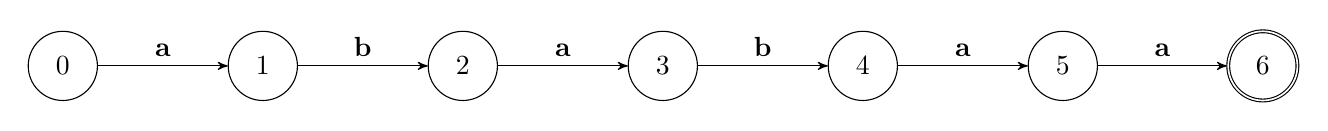
\begin{tikzpicture}
  % nodes
  \node [state] (0) {0};
  \foreach \n in {1, ..., 5} {
    \pgfmathtruncatemacro \p { \n - 1 };
    \node [state, right of = \p] (\n) {\n};
  }
  \node [state, accepting, right of = 5] (6) {6};
  \foreach \char [count = \n] in {a, b, a, b, a, a} {
    \pgfmathtruncatemacro \p { \n - 1 };
    \draw (\p) edge [above] node {\bf\char} (\n);
  }
\end{tikzpicture}
\end{document}
